
\paragraph{2. Additional \textit{happens-before} relations}
    Although we have identified the cases when \textit{happens-before} relations are preserved, we also get some additional relations in some of them.

    %Show an example here and explain
    As an example, for the case when $d$ is a sequentially consistent read, by lemma 1, in any execution of $C$
    \[
        \reln{k}{hb}{d} \centernot\Rightarrow \reln{k}{hb}{e} 
    \]

    But in $Executions$ of candidate $C'$, by transitivity, we have 
    \[
        \reln{k}{hb}{d} \Rightarrow \reln{k}{hb}{e} 
    \]

    This is because, there are sets of relations that come through \textit{synchronize-with} relations that $d$ has. Thus, although we are able to preserve relations that existed in any $Candidate Execution$ of $C$, we also in the process, introduce new ones in $Candidate Executions$ of $C'$. The figure below shows pictorially an example of a Candidate Execution of $C$ for the case above 

    %Show figure here of program P 
    \begin{figure}[H]
        \centering
        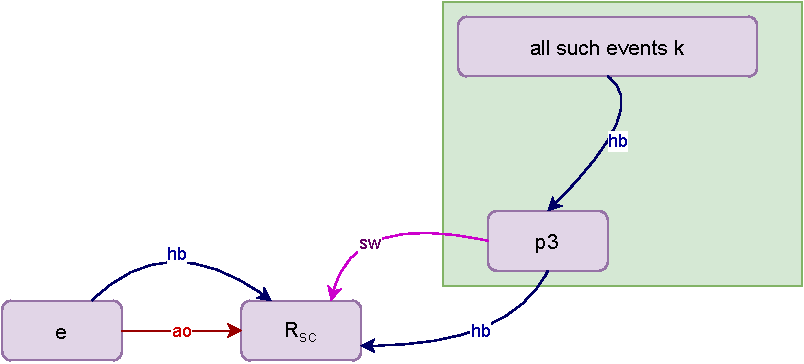
\includegraphics[scale=0.7]{Q2(c).pdf}
        \caption{A Candidate Execution where $d$ is a sequentially consistent read}
        \label{fig:my_label}
    \end{figure}

    %Show figure here of program P'
    \begin{figure}[H]
        \centering
        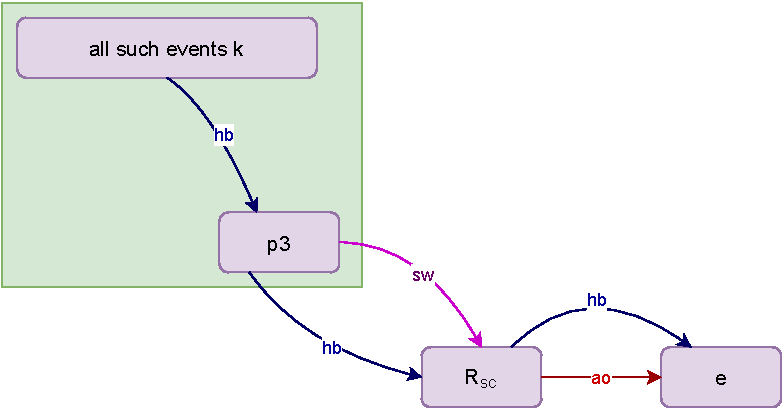
\includegraphics[scale=0.7]{Q2(d).pdf}
        \caption{The Candidate Execution after reordering, exposing the new relations established with $e$, $p3$ and set $k$}
        \label{fig:my_label}
    \end{figure}

    \critic{purple}{Explain the above figures or perhaps highlight the new relations that are established.}


    To summarize, the table below shows the cases where new relations could be introduced. 
    %Show the table here
    \begin{figure}[H]
        \centering
        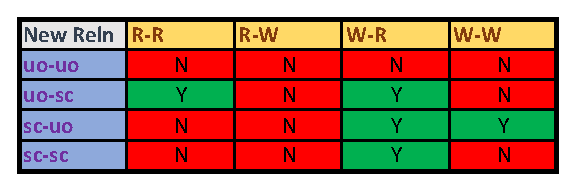
\includegraphics[scale=0.7]{Table2_Final.pdf}
        \caption{Table summarizing when new \textit{happens-before} relations could be introduced based on having valid pair of pivots }
        \label{fig:my_label}
    \end{figure}

    For these cases, we must know whether these new relations introduce new observable behaviors. 
